\documentclass[twocolumn, linenumbers]{aastex62} % preprint2

% CUSTOM PACKAGES AND COMMANDS
% ==============================
% CUSTOM PACKAGES
% =================
\usepackage[shadow]{todonotes}	% \todo{}: side notes at the margins; \todo[inline]{}: inline notes; \missingfigure{}; \listoftodos
\usepackage{color, soul}	% Highlighting, use \hl{...}
\usepackage{wrapfig}	% wrap text around figures; https://en.wikibooks.org/wiki/LaTeX/Floats,_Figures_and_Captions
\usepackage{verbatim}	% comment out chunks of text
\usepackage[normalem]{ulem} % fancy underlining, strikethrough spanning pages. \sout strikethrough, \xout, \underline



% Aliases and new definitions
% =============================

\newcommand{\vdag}{(v)^\dagger}
\newcommand\aastex{AAS\TeX}
\newcommand\latex{La\TeX}

% Symbol: Approximately proportional to (http://tex.stackexchange.com/questions/33538/how-to-get-an-approximately-proportional-to-symbol)
\def\apropto{%
  \def\p{%
    \setbox0=\vbox{\hbox{$\propto$}}%
    \ht0=0.6ex \box0 }%
  \def\s{%
    \vbox{\hbox{$\sim$}}%
  }%
  \mathrel{\raisebox{0.7ex}{%
      \mbox{$\underset{\s}{\p}$}%
    }}%
}

\newcommand{\fermi}{\emph{Fermi}}

\newcommand{\nemmen}{{\bf NEMMEN, R. S.}}

\newcommand{\lat}{\emph{Fermi} LAT Collaboration}

\newcommand{\continue}{\todo[inline,color=RedOrange]{
\centerline{ \textbf{\Large CONTINUE} }   
} }

\newcommand{\mario}{
\begin{wrapfigure}{l}{0.03\textwidth}
\vspace{-20pt}
\begin{center}

\includegraphics[width=0.07\textwidth]{figures/Mario.png}
\end{center}
\vspace{-10pt}
\end{wrapfigure}
}

\newcommand{\bowser}{
\begin{wrapfigure}{l}{0.03\textwidth}
\vspace{-20pt}
\begin{center}
\reflectbox{

\includegraphics[width=0.07\textwidth]{figures/Bowser.png}
}
\end{center}
\vspace{-10pt}
\end{wrapfigure}
}

% Environment for pretty box with title. Colors inspired
% on default style used in http://www.lasca.ic.unicamp.br/pub/ctan/macros/latex/contrib/tcolorbox/tcolorbox.pdf
% Usage: 
% \begin{boxed}{Box title}
% This is the text formatted by the boxed environment
% \end{boxed}
\definecolor{boxback}{HTML}{DAE5F0}
\definecolor{boxframe}{HTML}{0F365B}
\newenvironment{boxnamed}[1]
{   
\begin{tcolorbox}[enhanced, drop shadow, colframe=boxframe, colback=boxback,title=#1]
}
%text goes here
{
\end{tcolorbox}   
}

% Footnote without marker, cf. http://tex.stackexchange.com/questions/30720/footnote-without-a-marker
\newcommand\orphanfoot[1]{
  \begingroup
  \renewcommand\thefootnote{}\footnote{#1}
  \addtocounter{footnote}{-1}
  \endgroup
}

% figshare
\newcommand{\figshare}{fig\textbf{share}}

% cross (wrong) symbol, needs pifont package
\newcommand{\xmark}{\ding{56}}

% OK symbol (check), needs pifont package
\newcommand{\ok}{\ding{52}}

% Useful for citations with e.g.
\newcommand{\eg}[1]{(e.g. \citealt{#1})}

% fonts for code sample: \code{text sample}
\def\code#1{\texttt{#1}}

% red underline
\def\redul#1{{\color{red} \underline{\color{black}#1}}}







% PAPER PREAMBLE
% ===================
\received{May 4, 2019}
\revised{June 4, 2019}
\accepted{\today}
\submitjournal{ApJL}
%\AuthorCollaborationLimit=3
%% Use \allauthors at the manuscript end to show the full author list.
%% This command should only be used when \AuthorCollaborationLimit is used.

\shorttitle{Spin of M87*}
\shortauthors{Nemmen}
%\watermark{DRAFT} % adds a light gray and diagonal water-mark to the first page. If the text is long you can control the water-mark size with: \setwatermarkfontsize{dimension}






% BEGINNING OF MANUSCRIPT / PAPER CONTENT
% ==========================================
\begin{document}

\title{The Spin of M87*}



%\correspondingauthor{Rodrigo Nemmen}
\email{rodrigo.nemmen@iag.usp.br}

\author{Rodrigo Nemmen}
\affil{Universidade de S\~ao Paulo, Instituto de Astronomia, Geof\'{\i}sica e Ci\^encias Atmosf\'ericas, Departamento de Astronomia, S\~ao Paulo, SP 05508-090, Brazil}
%\collaboration{(Fermi LAT Collaboration)}
\nocollaboration




\begin{abstract}
Now that the mass of central black hole in the galaxy M87 has been measured by imaging the shadow of the event horizon, the remaining parameter of the Kerr metric that needs to be estimated is the spin $a_*$. We have modeled the measurements of the power of the relativistic jet and the black hole mass accretion rate with general relativistic magnetohydrodynamic models of jet formation. This allows us to derive constraints on $a_*$ and the black hole magnetic flux $\phi$. We find a lower limit on M87*'s spin and magnetic flux of $|a_*| \geq 0.4$ and $\phi \gtrsim 6$ in the prograde case, and $|a_*| \geq 0.5$ and $\phi \gtrsim 10$ in the retrograde case, otherwise the black hole is not able to provide enough energy to power the observed jet. These results disfavor a variety of models typified by low values of $\phi$ known as ``SANE''. This suggests that M87* prefers the magnetically arrested disk state. 
\end{abstract}

\keywords{keywords}





\section{Introduction} \label{sec:intro}

The shadow cast by the event horizon of a black hole (BH) has been imaged for the first time with the Event Horizon Telescope (EHT) for the supermassive black hole (SMBH) at the center of the galaxy M87, known as M87* (\citealt{EHTC2019}, hereafter EHTC). The very long baseline interferometry (VLBI) observation at a wavelength of 1.3 mm of the asymmetric bright emission ring gives an angular diameter of $d=42 \pm 3 \ \mu$as, which allows an unprecedented constraint on the SMBH mass of $M=(6.5 \pm 0.7) \times 10^9 M_\odot$--the first fundamental parameter of the \cite{Kerr1963} metric. The inferred mass is in agreement with--and hence strongly favors--the mass measurement based on stellar dynamics \citep{Gebhardt2011}. 

However, the second parameter of the Kerr metric--the dimensionless spin $a_* \equiv Jc/GM^2$ where $J$ is the angular momentum of the black hole--is much harder to constrain with shadow observations. The reason is that the ring diameter has a very weak dependence on $a_*$ or the disk inclination, varying by only 4\% in the range $a_*=0$ to $\approx 1$ \citep{Takahashi2004,Johannsen2010}. Measuring the ring properties with precision enough to set useful constraints on the spin may require VLBI at shorter wavelengths, more telescopes or space-based interferometry (e.g., EHTC, \citealt{Roelofs2019}).

Besides mass and spin, black hole accretion is also described by two other parameters: the mass accretion rate onto the BH $\dot{M}$ and the magnetic flux $\Phi$ crossing one hemisphere of the event horizon. In this Letter, we set bounds on the values of $a_*$ and $\Phi$ of M87* by modeling the energetics of its relativistic jet as being powered by the Blandford-Znajek process--the extraction of BH spin energy through electromagnetic torques. The observational input to our estimates are the measurements of $M$, $\dot{M}$ and the power carried by the jet. We assume a distance to M87* of 16.8 Mpc (e.g.,  \citealt{Blakeslee2009, EHTC2019e}; hereafter EHTC5). At this distance, cosmological effects are negligible. 
% FURTHERMORE, IT IS RELEVANT TO ALSO CONSTRAIN ANOTHER PARAMETER OF INTEREST, THE MAGNETIC FLUX WHICH IS IMPORTANT FOR JET PRODUCTION




\section{Observations} \label{sec:obs}

In this work, the fundamental quantity needed in order to constrain the BH spin in M87* is the efficiency of jet production $\eta \equiv P/ \dot{M} c^2$, where $P$ is the power carried by the relativistic jet--the jet power--and $\dot{M}$ is the mass accretion rate onto the SMBH. Therefore, $P$ and $\dot{M}$ are the M87* observables that we need in order to apply our models of jet production to constrain the spin parameter.

% Jet power from Cavity power \cite{Russell2013}
There are different ways of measuring the jet power of M87, with  different methods giving powers in the range $P \sim 10^{42}-10^{45} \ {\rm erg \ s}^{-1}$ (e.g., \citealt{Reynolds1996, Allen2006, Abdo2009, Degasperin2012, Nemmen2014}; cf. EHTC5 and references therein). Here, we use the jet-inflated X-ray cavities observed in the central regions of M87 with the \textit{Chandra} X-ray Telescope as calorimeters to estimate the jet power \citep{Russell2013}. The jet power was estimated as $P = E_{\rm cav}/t_{\rm age}$, where $E_{\rm cav}$ is the energy required to create the observed cavities and $t_{\rm age}$ is the age of the cavity. The usual assumption in deriving $E_{\rm cav}$ is that the cavities are inflated slowly such that $E_{\rm cav}=4PV$ where $P$ is the thermal pressure of the surrounding X-ray emitting gas, $V$ is the volume of the cavity and the cavity is assumed to be filled up with relativistic plasma. %The age of the cavity is usually assumed to be either the sound-crossing timescale $t_{\rm c_s}$ where $D$ is the distance of the bubble centre from the black hole and $c_s$ is the adiabatic sound speed, or the buoyancy timescale $t_{\rm buoy}=D/v_t$ where $v_t$ is the bubble terminal velocity. 
This method of measuring $P$ is well-established and robust \eg{Birzan2004, Dunn2004, McNamara2012, Hlavacek2013}, giving the jet power averaged over the timescale during which the central engine produces one continuous pair of jets. We believe this is the most direct way of measuring the jet power and therefore accept the X-ray cavity power at face value as M87's jet power, $\log P = 42.9^{+0.2}_{-0.27} \ {\rm erg \ s}^{-1}$. 
% cf. Nemmen+2015 for a detailed discussion of this method of estimating jet powers

% Mass accretion rate by \cite{Kuo2014}
For the mass accretion rate onto the BH, we use the constraint obtained by \cite{Kuo2014} based on the Faraday rotation measure (RM) observed with the Submillimeter Array. Kuo et al. measured the M87*'s RM at four  frequencies around 230 GHz to be in the range $−7.5 \times 10^5-3.4 \times 10^5 \ {\rm rad \ m}^{-2}$. By making reasonable assumptions, Kuo et al. estimated the upper limit $\dot{M} (42 r_g) \leq 9.2 \times 10^{-4} \ M_\odot \ {\rm yr}^{-1}$ where $\dot{M} (42 r_g)$ is the mass accretion rate at a distance of 42 gravitational radii from the SMBH ($r_g \equiv GM/c^2$). The corresponding accretion power is $\log (\dot{M} (42 r_g) c^2) = 43.7 \ {\rm erg \ s}^{-1}$. The question is of course how to connect this measurement with the accretion rate $\dot{M}$ near the event horizon. We will come back to this question in section \ref{models}.

% ?density profile by \cite{Russell2018}?





\section{Models}    \label{models}

The leading idea to understand how accreting Kerr BHs produce relativistic jets is the Blandford-Znajek process \citep{Blandford1977, Blandford2019}. According to this mechanism, the rotating event horizon is threaded by large-scale magnetic field lines, which were brought in together with accreted gas. %The BH exerts a torque on the field lines and progressively loses rotational energy to its environment. This spin energy is converted to a Poynting flux-dominated outflow \eg{McKinney2004,DeVilliers2005} which eventually transfers the electromagnetic energy to particles in the relativistic jet. 
The BH exerts a torque on the field lines and progressively transfers its rotational energy to the relativistic jet \eg{McKinney2004,Semenov2004}. According to the Blandford-Znajek model, the jet power depends on $a_*$ and the magnetic flux $\Phi$ threading the horizon as $P \propto ( a_* \Phi/M )^2$ to first order \citep{Blandford1977}. In reality, for rapidly spinning BHs the jet power depends in a more complicated nonlinear fashion on the spin as higher-order spin corrections become important \eg{Sasha2010}. 

We use the results of global, general relativistic magnetohydrodynamic (GRMHD) simulations of radiatively inefficient accretion flows (RIAFs; \citealt{Yuan2014}) around Kerr BHs to model the dependence of the jet power on $a_*$ and $\Phi$. Concretely, we model the jet power as $P = \eta(a_*, \Phi) \dot{M} c^2$ where the jet production efficiency 
\begin{equation}
\eta = \left( \frac{\phi}{15} \right)^2 f(a_*)
\end{equation}
is a function of both the spin and dimensionless magnetic flux $\phi \equiv \Phi/(\dot{M} r_g^2)^{1/2}$. We use the GRMHD results of \cite{Sasha2012a}--which used the \code{HARM} code \citep{Gammie2003}--to set the spin-dependence of $\eta$. \cite{Sasha2012a} carried out RIAF simulations in the ``magnetically arrested disk'' (MAD) limit, for which the magnetic flux saturates at $\phi \sim 15$ \citep{Narayan2003, Sasha2011}, with $h/r \approx 0.3$ where $h$ is the disk thickness. In order to consider the full range of astrophysically relevant magnetic fluxes, we also take into account the case of  ``standard and normal disk evolution'' (SANE) with $\phi \sim 1$ \eg{Narayan2012}. Figure  \ref{spin-model} illustrates the spin-dependence of the $\eta$. Notice that this model encompasses both the prograde and retrograde cases in which the disk and BH are rotating in the same and opposite senses, respectively. Retrograde BHs produce less powerful jets \citep{Sasha2012}.

\begin{figure}[h]
\centering
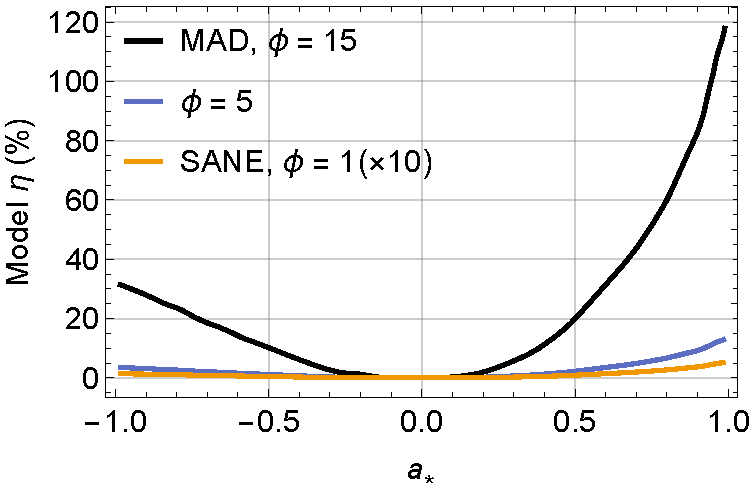
\includegraphics[width=\linewidth]{figures/model-eta.pdf}
\caption{The efficiency of the jet production efficiency $\eta$ as a function of the black hole spin $a_*$ from GRMHD simulations of RIAFs, for different values of the magnetic flux $\phi$. Both prograde ($a_*>0$) and retrograde ($a_*<0$) cases are encompassed. The SANE model $\eta$-values were multiplied by 10. }
\label{spin-model}
\end{figure}

In order to connect the accretion rate at $r=42 r_g$ constrained by the Faraday RMs of \cite{Kuo2014} with the BH rate, we adopt the simple radial scaling $\dot{M}(r) = \dot{M_0} (r/r_0)^s$ originally proposed as an ansatz by \cite{Blandford1999} in their ``ADIOS'' model--and later supported by many global simulations \eg{Yuan2015}. This $\dot{M}(r)$ scaling corresponds to a density radial profile $\rho(r) \propto r^{-\beta}$ where $\beta = 3/2-s$. We define the BH accretion rate as $\dot{M}(6 r_g)$ so we fix $r=6r_g$, $r_0=42 r_g$ and $\dot{M}_0$ as the accretion rate constrained by Kuo et al. We want to be agnostic regarding the variety of possible density profiles in M87*, therefore we allow $\beta$ ($s$) to vary in the range $1.5-0.5$ ($0-1$), i.e. allowing for different levels of mass-loss in the RIAF. We should note that \cite{Russell2018}  measured $\beta \approx 1.5$ at $r=(0.1-1)$ kpc in M87, which is outside but very close to the Bondi radius ($r_B = 0.03$ kpc). 






\section{Results} 

Our first result is a model-independent estimate of the jet production efficiency from the SMBH in M87* from the observed jet power and mass accretion rate while allowing a variety of density profiles as described in the previous section. Figure \ref{obs-eta} shows this result, with $\eta$ varying from $\approx 10\%$ ($1\sigma$ lower limit, $\beta=1.5$) up to about $200\%$ ($1\sigma$ upper limit, $\beta=0.5$) if the density profile flattens towards the BH.

\begin{figure}[h]
\centering
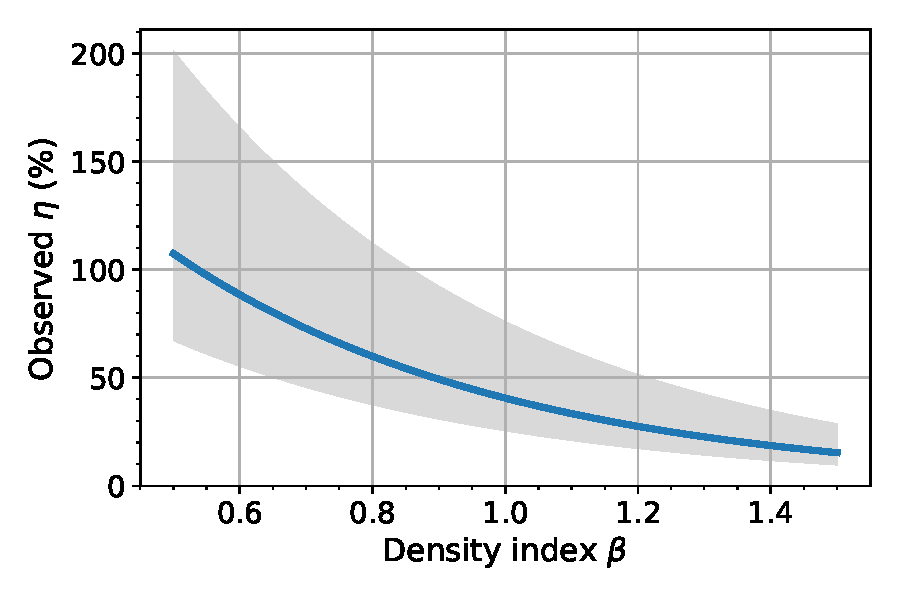
\includegraphics[width=\linewidth]{figures/observed-eta.pdf}
\caption{Observed jet production efficiency $\eta_{\rm observed}$ for M87* as a function of $\beta$ ($\rho \propto r^{-\beta}$). The shaded area represents the $1\sigma$ uncertainty propagated from the uncertainty in the observed jet power. }
\label{obs-eta}
\end{figure}

With the considerations in the previous section, we have a model that provides a full mapping of the observed jet efficiency derived above to the spin and magnetic flux 
\begin{equation}    \label{eq}
\eta_{\rm observed}=\eta(a_*, \phi).
\end{equation}
We proceed by solving this nonlinear equation, using the values of $\eta_{\rm observed}$ displayed in Figure \ref{obs-eta} to constrain the physical parameters of the event horizon beyond its mass--assuming that the Kerr metric is the correct description of the spacetime. Figure \ref{spins} shows the inferred spin of M87* on the assumption that the SMBH is in the MAD state--i.e. with the maximum value of $\phi$. 

The lessons behind Fig. \ref{spins} are the following: (i) If M87* is in the MAD state then the only allowed spins are $a_* \leq -0.5$ or $a_* \gtrsim 0.4$ (within the $1\sigma$ uncertainty bands). (ii) If the density profile of the accretion flow follows $\rho \propto r^{-1.5}$ as in RIAF models without mass-loss \eg{Narayan1994}, then $a_* = 0.45^{+0.12}_{-0.08}$ (prograde) or $a_* = -0.62^{+0.14}_{-0.30}$ (retrograde). (iii) If the BH is retrograde then values of $\beta \geq 0.9$ are favored otherwise M87* would not be able to power its jet through the Blandford-Znajek process; all values of $\beta$ are allowed if the BH is prograde.
Notice that we limit the upper value of $|a_*|$ to one because the BH solution is not valid anymore above this limit.

\begin{figure}[h]
\centering
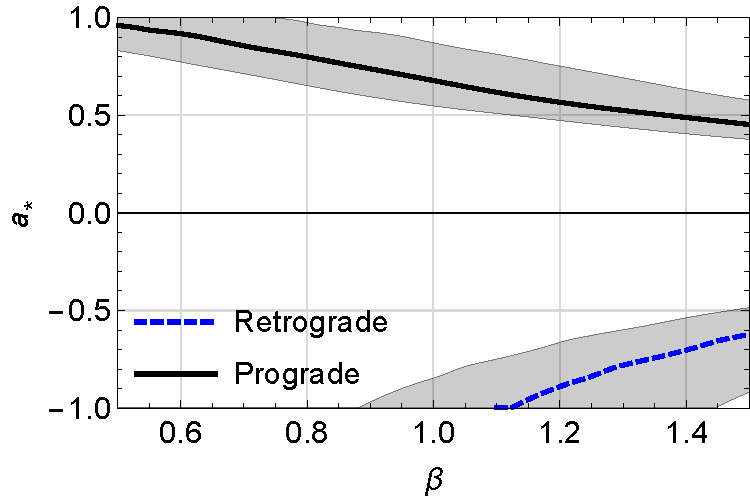
\includegraphics[width=\linewidth]{figures/spins-MAD.pdf}
\caption{The spin of the SMBH in M87* as a function of $\beta$ for both the prograde and retrograde cases, assuming that it is in the MAD state. The shaded region corresponds to the $1\sigma$ uncertainty band around the mean. The uncertainty was propagated from the uncertainty in the observed jet powers. }
\label{spins}
\end{figure}

Figure \ref{spins-phi} shows the solutions of the equation \ref{eq} for $a_*$ and $\phi$ that are consistent with the mean values of $\eta_{\rm observed}$ (i.e. the values along the solid line in Fig. \ref{obs-eta}). %, for different possibilities of density profiles parameterized as a range of values of $\beta$. 
As such, Fig. \ref{spins-phi} gives us the observational constraints on M87*'s spin and magnetic flux. To begin with, the hatched area in the plot indicates the region of the parameter space which is forbidden for M87* on the assumption of the Kerr metric, because they would imply $|a_*| > 0.998$ which is the astrophysical limiting value of the spin \citep{Thorne1974}. In other words, in the hatched region the SMBH does not provide enough energy to power the observed jet. We now describe separately the prograde and retrograde cases. The MAD state corresponds to the top part of the plot ($\phi \approx 15$) while the SANE mode with $\phi \sim 1$--as considered among the models in EHTC5--corresponds to the bottom region. \\
%
\textbf{Prograde.} In this case, not all magnetic fluxes are accessible to the SMBH. For instance, only accretion flows with $\phi \gtrsim 6$ are possible. In the extreme situation that $\beta=0.5$  the RIAF must be in the MAD state. All values of $\beta$ are allowed. \\
\textbf{Retrograde.} Retrograde BHs produce less powerful jets, therefore if the SMBH is retrograde this implies tighter constraints on M87*'s parameters compared to the prograde case. Only RIAFs with  $\phi \gtrsim 10$ and $\beta \gtrsim 1.1$ are possible.  \\

\begin{figure*}
    \centering
    \begin{minipage}{0.45\textwidth}
        \centering
        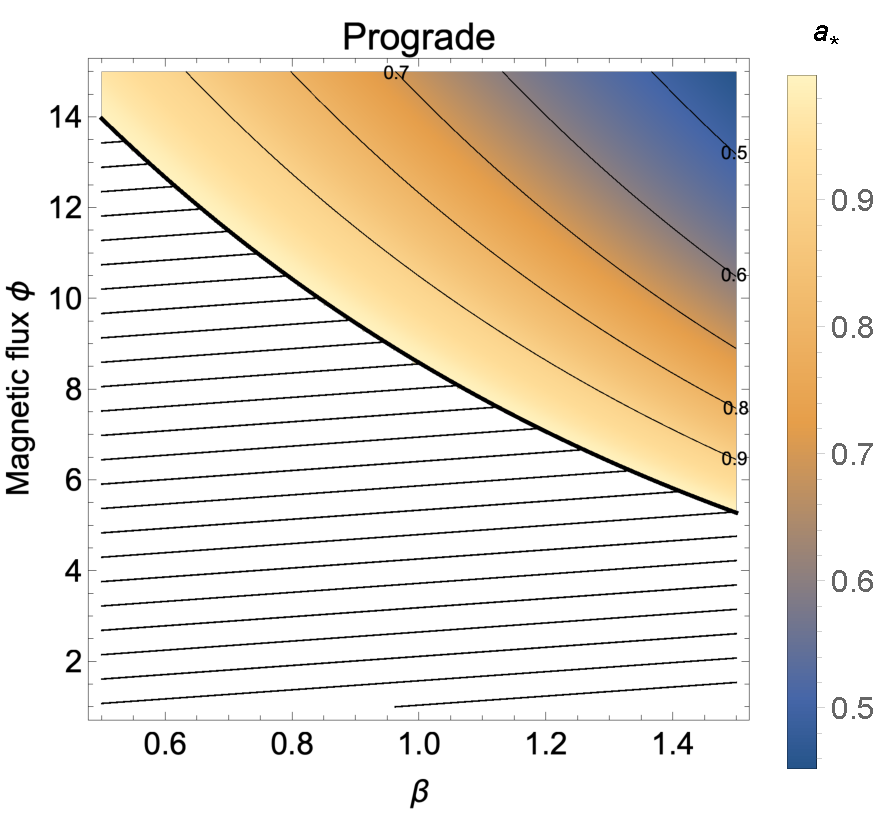
\includegraphics[width=\textwidth]{figures/phi-beta-spins-prograde.pdf} % first figure itself
    \end{minipage}\hfill
    \begin{minipage}{0.45\textwidth}
        \centering
        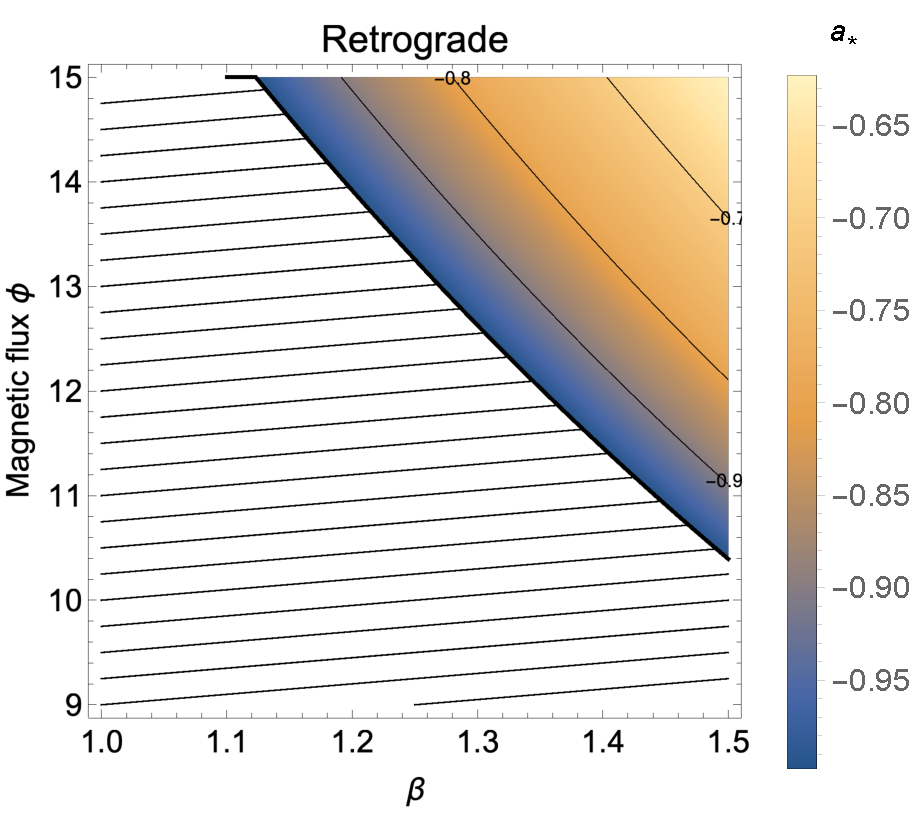
\includegraphics[width=\textwidth]{figures/phi-beta-spins-retrograde.pdf} % second figure itself
    \end{minipage}
\caption{Observational parameter space for M87*--spin, magnetic flux and $\beta$--consistent with the average observed jet power. The left and right panels display the prograde and retrograde SMBH cases, respectively. The MAD and SANE states correspond to the top and bottom part of the plots, respectively. The hatched region indicates parameters which are forbidden to the SMBH because they would imply  $|a_*|>0.998$. }
\label{spins-phi}
\end{figure*}




\section{Discussion} \label{sec:disc}

% does this rule out any models for consideration, based on the jet energetics?
Our results are fundamentally based on the modeling of $\eta_{\rm observed}$--the observationally constrained jet production efficiency of M87*. We compute $\eta_{\rm observed}$ from the jet power measured from the X-ray cavities and BH accretion rate upper limit measured from Faraday RMs. From our modeling of $\eta_{\rm observed}$, we rule out a considerable region of the BH accretion parameter space for M87*. In particular, we have found that all SANE models with $\phi \sim 1$--i.e. the family of SANE models considered in EHTC, EHTC5--are inconsistent with the jet energetics since their magnetic flux gives very small jet efficiencies. Most of the MAD models considered in EHTC5 are consistent with our $\phi$-constraints, except those with $\phi \approx 8$ and $a_*<0$.

% why the difference between efficiencies in our work and paper V?
It is interesting to discuss one notable difference between our results and those of EHTC5. The SANE models with $\phi \approx 1$ and $a_*=-0.94$ simulated by EHTC5 are characterized by low jet efficiencies $\eta = 5 \times 10^{-3}$, therefore they do not agree with the observational efficiency constraints $\eta_{\rm observed} > 0.1$. However, they produce jet powers in the range $P \sim 10^{42}-10^{43} \ {\rm erg \ s}^{-1}$ which are comparable to the observations and therefore pass the ``jet power consistency test'' performed in EHTC5. What is the origin of this apparent contradiction between the simulated large $P$ and low $\eta$ for these models? 
% mdot here < 6.17e-6 mdot_Edd
% my mdot is less model-dependent 
The root of the contradiction are the values of $\dot{M}$ from the GRMHD simulations: they are model-dependent and span a wide range, e.g. they depend on the parameter $R_{\rm high}$ \citep{Moscibrodzka2016}. By contrast, in our work we base $\dot{M}$ on the Faraday RM measurement at $42 r_g$ \citep{Kuo2014} and allow it be smaller depending on the RIAF density profile (\textsection \ref{models}). We think our choice of $\dot{M}$ for M87* is less model-dependent. 

Concretely, the SANE models of EHTC5 with $\phi \approx 1$ and $a_*=-0.94$ have accretion rates larger than the upper limit on $\dot{M}$ adopted in this work by a factor of $4-47$; these larger $\dot{M}$s result in larger jet powers even though their $\eta$s are comparable to ours (our model gives $\eta(-0.94, 1.02) \approx  1.4 \times 10^{-3}$). Interestingly enough, their SANE models with $\phi = 1.64$ and $a_*=0.94$ have $\dot{M}$ comparable to the upper limit adopted in this work and similar efficiencies, and not surprisingly these GRMHD models give jet powers much weaker than the observations, in agreement with our results.
% \eta(+0.94, 1.64) = 0.018 here vs 7.76e-3 in EHTC5

% comparisons with other work
%- Compare with constraints of EHTC paper 5
%- compare with previous constraints. other papers...

% Caveats
One assumption of our work is that the $\eta$ dependency on the BH parameters is adequately described by global ideal GRMHD simulations of relativistic jet formation. These models have achieved an impressive level of sophistication in the last few years and the results of different GRMHD codes broadly agree with each other \eg{Porth2019}. However, simulations which incorporate departures from the MHD approximation are suggesting that jet formation can be more complex than previously thought \citep{Parfrey2019}. Furthermore, we have only considered the case of a BH spin vector aligned with the angular momentum vector of the accretion flow. The general case of arbitrary relative orientations of these vectors can lead to more complicated jet behaviors \citep{Liska2018}. These issues deserve further investigations. 

% how does this impact the shadow?
Finally, as we already mentioned the BH shadow is weakly affected by the different values of $a_*$ and it is not clear whether further EHT observations will eventually be able to constrain the ring properties with enough sharpness to meaningfully constrain the spin. We are looking forward to advancements in VLBI techniques that will potentially advance our understanding of M87*'s spin (e.g. going to shorter wavelengths, adding more telescopes, going to space-based interferometry; e.g. \citealt{Roelofs2019}) and also to upcoming polarimetric analysis of the EHT observations which will further constrain the magnetic flux and accretion rates.




\section{Summary}	\label{sec:summary}

We have assembled multiwavelength observations of M87 which constrain the power carried by particles in the relativistic jet through X-ray imaging and the black hole mass accretion rate through radio polarization. Comparing these observables with the predictions of GRMHD models of jet formation allows us to derive constraints on the spin and magnetic flux of M87*'s supermassive black hole. Our main conclusions can be summarized as follows:

(i) The black hole in M87* is converting at least $\eta=10\%$ of the accreted rest mass energy to jet power, and up to $200\%$ depending on how shallow the density profile of the accretion flow is.

(ii) We derive a robust lower limit on M87*'s spin: $|a_*| \geq 0.4$ in the prograde case or $|a_*| \geq 0.5$ in the retrograde case. We are not able to distinguish between the prograde or retrograde scenarios based only on the data we have used.
%of the SMBH if it is in the MAD state accreting with $\rho \propto r^{-1.5}$:  

(iii) We obtained lower limits on the BH magnetic flux, potentially ruling out a variety of models with low values of $\phi$ known as ``SANE''. We find that $\phi \gtrsim 6$ in the prograde case and $\phi \gtrsim 10$ in the retrograde case. Therefore, the magnetically arrested disk state seems to be preferred by M87*.

%density profiles ruled out...

We hope that these constraints on the M87*'s black hole spin and magnetic flux will be useful in further extracting physical parameters from M87*'s BH shadow.




\acknowledgments

We would like to thank Sasha Tchekhovskoy for providing us with the electronic data for his GRMHD simulations in a convenient format. 
%We acknowledge useful discussions with Roderik Overzier. 
This work was supported by FAPESP (Funda\c{c}\~ao de Amparo \`a Pesquisa do Estado de S\~ao Paulo) under grant 2017/01461-2. The Black Hole Group at USP has received a generous donation of a GPU from NVIDIA under the GPU Grant Program.

\vspace{5mm}
\facilities{\textit{Chandra} X-ray Observatory, Submillimeter Array, Event Horizon Telescope}
\software{Jupyter \citep{ipython}, \href{https://github.com/tisimst/mcerp}{\code{mcerp}},   \href{https://github.com/rsnemmen/nmmn}{\code{nmmn}}} % specifies which programs were used



\appendix

\section{Appendix information}



% REFERENCES
% ============
\bibliography{refs}

%\allauthors % shows entire author+affilation list. Has to go at the end of the manuscript

%% Include this line if you are using the \added, \replaced, \deleted
%% commands to see a summary list of all changes at the end of the article.
%\listofchanges

\end{document}